\documentclass[11pt,a4paper]{article}
\usepackage[T1]{fontenc}
\usepackage[utf8]{inputenc}
% \usepackage[french]{babel}  % Commenté pour compatibilité
\usepackage[a4paper, margin=2.5cm]{geometry}
\usepackage{amsmath, amssymb}
\usepackage{siunitx}
\usepackage{booktabs}
\usepackage{float}
\usepackage{tikz}
\usepackage{tikz-3dplot}
\usepackage[most]{tcolorbox}
\usepackage{caption}
\usepackage{subcaption}

\usetikzlibrary{positioning, arrows.meta, shapes.geometric, patterns, decorations.pathreplacing, calc, 3d}

% Couleurs personnalisees
\definecolor{wpetg}{RGB}{34,139,34}
\definecolor{aircolor}{RGB}{200,230,255}
\definecolor{billeA}{RGB}{218,165,32}
\definecolor{billeB}{RGB}{205,92,92}
\definecolor{watercolor}{RGB}{100,180,255}
\definecolor{enveloppe}{RGB}{230,230,230}
\definecolor{detector}{RGB}{100,100,255}

\title{\textbf{Description de la Geometrie Geant4}\\[0.5cm]
\Large Plaque W/PETG avec Cavite d'Air et Empilement de Billes de Bismuth}
\author{Documentation Technique}
\date{\today}

\begin{document}

\maketitle

\begin{tcolorbox}[colback=blue!5, colframe=blue!70!black, title=\textbf{Resume}]
Ce document presente la geometrie d'une simulation Geant4 comprenant :
\begin{itemize}
    \item Une plaque de W/PETG (75\%/25\%) de 18 mm d'epaisseur
    \item Une cavite d'air centrale (50$\times$50$\times$8.53 mm$^3$)
    \item Un empilement hexagonal compact de 5 plans de billes de bismuth ($\sim$3449 billes)
    \item Un detecteur de dose spherique (eau) a 20 cm de la source
\end{itemize}
\end{tcolorbox}

\tableofcontents
\newpage

%==============================================================================
\section{Vue d'Ensemble de la Geometrie}
%==============================================================================

\subsection{Schema Global}

La figure~\ref{fig:vue_ensemble} presente une vue d'ensemble de la geometrie le long de l'axe $z$ (axe du faisceau).

\begin{figure}[H]
\centering
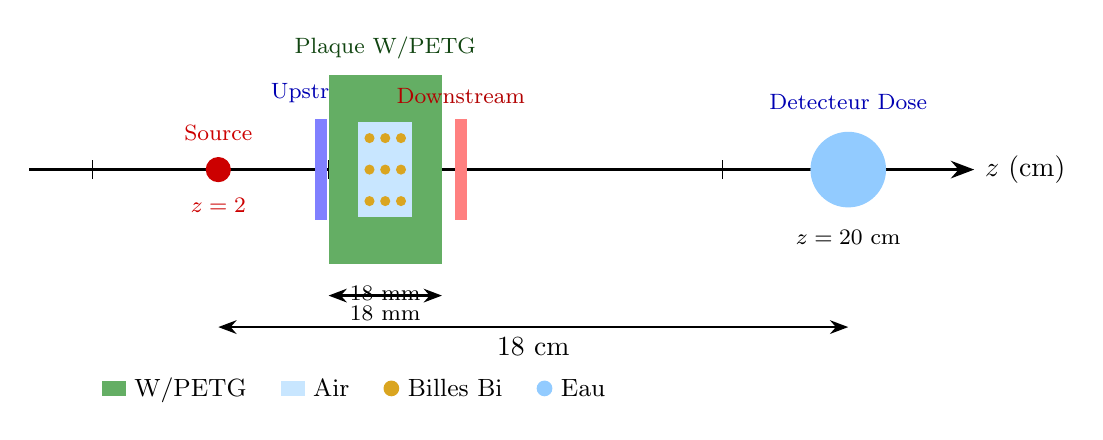
\begin{tikzpicture}[scale=0.8, >=Stealth]

% Axe Z
\draw[->, very thick] (-1,0) -- (14,0) node[right] {$z$ (cm)};

% Marques sur l'axe
\foreach \x/\label in {0/0, 2/2, 3.75/3.75, 4.65/4.65, 5.55/5.55, 10/10, 12/12} {
    \draw (\x, -0.15) -- (\x, 0.15);
}

% Source (z = 2 cm)
\fill[red!80!black] (2, 0) circle (0.2);
\node[above, red!80!black] at (2, 0.3) {\footnotesize Source};
\node[below, red!80!black] at (2, -0.3) {\footnotesize $z=2$};

% Upstream detector (z = 3.53 cm)
\fill[blue!50] (3.53, -0.8) rectangle (3.73, 0.8);
\node[above, blue!70!black, font=\footnotesize] at (3.63, 0.9) {Upstream};

% Plaque W/PETG avec cavite
\fill[wpetg!70] (3.75, -1.5) rectangle (5.55, 1.5);
% Cavite d'air
\fill[aircolor] (4.22, -0.75) rectangle (5.08, 0.75);
% Billes (symboliques)
\foreach \y in {-0.5, 0, 0.5} {
    \fill[billeA] (4.4, \y) circle (0.08);
    \fill[billeA] (4.65, \y) circle (0.08);
    \fill[billeA] (4.9, \y) circle (0.08);
}

\node[above, wpetg!50!black, font=\footnotesize] at (4.65, 1.6) {Plaque W/PETG};
\node[below, font=\footnotesize] at (4.65, -1.7) {18 mm};

% Downstream detector (z = 5.75 cm)
\fill[red!50] (5.75, -0.8) rectangle (5.95, 0.8);
\node[above, red!70!black, font=\footnotesize] at (5.85, 0.9) {Downstream};

% Detecteur dose (z = 20 cm) - mis a l'echelle
\fill[watercolor!70] (12, 0) circle (0.6);
\node[above, blue!70!black, font=\footnotesize] at (12, 0.8) {Detecteur Dose};
\node[below, font=\footnotesize] at (12, -0.8) {$z=20$ cm};

% Cotations
\draw[<->, thick] (2, -2.5) -- (12, -2.5) node[midway, below] {18 cm};
\draw[<->, thick] (3.75, -2) -- (5.55, -2) node[midway, below] {\footnotesize 18 mm};

% Legende
\node[right, font=\small] at (0, -3.5) {
    \tikz{\fill[wpetg!70] (0,0) rectangle (0.3,0.2);} W/PETG \quad
    \tikz{\fill[aircolor] (0,0) rectangle (0.3,0.2);} Air \quad
    \tikz{\fill[billeA] (0.15,0.1) circle (0.1);} Billes Bi \quad
    \tikz{\fill[watercolor!70] (0.15,0.1) circle (0.1);} Eau
};

\end{tikzpicture}
\caption{Vue d'ensemble de la geometrie le long de l'axe $z$.}
\label{fig:vue_ensemble}
\end{figure}

\subsection{Parametres Geometriques}

\begin{table}[H]
\centering
\caption{Parametres geometriques principaux}
\begin{tabular}{llc}
\toprule
\textbf{Element} & \textbf{Parametre} & \textbf{Valeur} \\
\midrule
\multirow{4}{*}{Plaque W/PETG} 
    & Dimensions X $\times$ Y & $100 \times 100$ mm$^2$ \\
    & Epaisseur (Z) & 18 mm \\
    & Position centre & $z = 4.65$ cm \\
    & Densite & $\sim 4.5$ g/cm$^3$ \\
\midrule
\multirow{3}{*}{Cavite d'air}
    & Dimensions X $\times$ Y & $50 \times 50$ mm$^2$ \\
    & Hauteur (Z) & 8.53 mm \\
    & Position & Centree dans la plaque \\
\midrule
\multirow{4}{*}{Billes Bismuth}
    & Diametre & 2 mm \\
    & Nombre de plans & 5 \\
    & Nombre total & $\sim 3449$ \\
    & Densite Bi & 9.75 g/cm$^3$ \\
\midrule
\multirow{2}{*}{Detecteur Dose}
    & Rayon & 2 cm \\
    & Position & $z = 20$ cm \\
\bottomrule
\end{tabular}
\end{table}

\newpage

%==============================================================================
\section{Structure de la Plaque W/PETG}
%==============================================================================

\subsection{Vue en Coupe XZ}

La figure~\ref{fig:coupe_xz} presente une coupe verticale de la plaque montrant la cavite d'air et l'empilement de billes.

\begin{figure}[H]
\centering
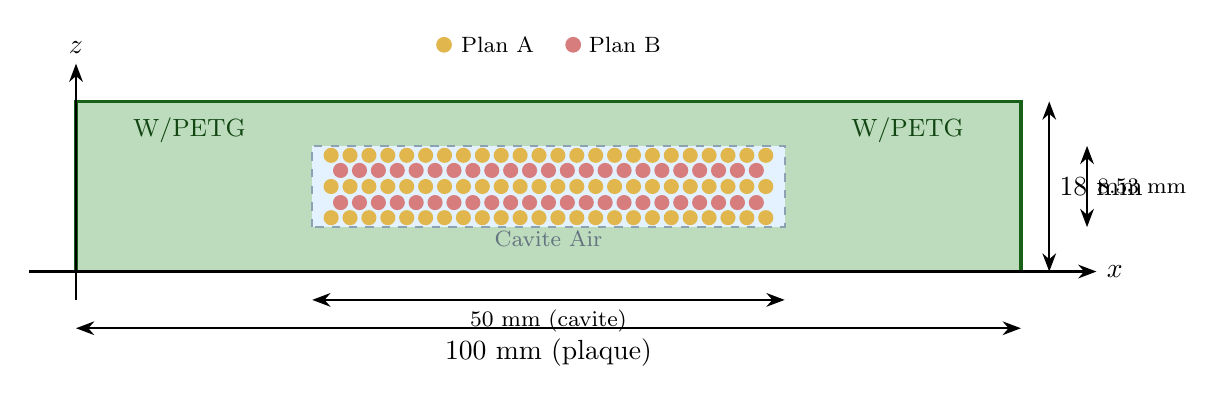
\begin{tikzpicture}[scale=1.2, >=Stealth]

% Cadre exterieur (plaque W/PETG)
\fill[wpetg!30] (-5, -0.9) rectangle (5, 0.9);

% Cavite d'air
\fill[aircolor!50] (-2.5, -0.43) rectangle (2.5, 0.43);

% Contour de la cavite
\draw[thick, dashed, aircolor!70!black] (-2.5, -0.43) rectangle (2.5, 0.43);

% Billes (5 plans)
\def\r{0.08}
\def\dz{0.163}

% Plan 1 (Type A) - z = -0.33
\foreach \x in {-2.3, -2.1, -1.9, -1.7, -1.5, -1.3, -1.1, -0.9, -0.7, -0.5, -0.3, -0.1, 0.1, 0.3, 0.5, 0.7, 0.9, 1.1, 1.3, 1.5, 1.7, 1.9, 2.1, 2.3} {
    \fill[billeA!80] (\x, -0.33) circle (\r);
}

% Plan 2 (Type B) - z = -0.17
\foreach \x in {-2.2, -2.0, -1.8, -1.6, -1.4, -1.2, -1.0, -0.8, -0.6, -0.4, -0.2, 0.0, 0.2, 0.4, 0.6, 0.8, 1.0, 1.2, 1.4, 1.6, 1.8, 2.0, 2.2} {
    \fill[billeB!80] (\x, -0.17) circle (\r);
}

% Plan 3 (Type A) - z = 0
\foreach \x in {-2.3, -2.1, -1.9, -1.7, -1.5, -1.3, -1.1, -0.9, -0.7, -0.5, -0.3, -0.1, 0.1, 0.3, 0.5, 0.7, 0.9, 1.1, 1.3, 1.5, 1.7, 1.9, 2.1, 2.3} {
    \fill[billeA!80] (\x, 0) circle (\r);
}

% Plan 4 (Type B) - z = 0.17
\foreach \x in {-2.2, -2.0, -1.8, -1.6, -1.4, -1.2, -1.0, -0.8, -0.6, -0.4, -0.2, 0.0, 0.2, 0.4, 0.6, 0.8, 1.0, 1.2, 1.4, 1.6, 1.8, 2.0, 2.2} {
    \fill[billeB!80] (\x, 0.17) circle (\r);
}

% Plan 5 (Type A) - z = 0.33
\foreach \x in {-2.3, -2.1, -1.9, -1.7, -1.5, -1.3, -1.1, -0.9, -0.7, -0.5, -0.3, -0.1, 0.1, 0.3, 0.5, 0.7, 0.9, 1.1, 1.3, 1.5, 1.7, 1.9, 2.1, 2.3} {
    \fill[billeA!80] (\x, 0.33) circle (\r);
}

% Contour de la plaque
\draw[very thick, wpetg!70!black] (-5, -0.9) rectangle (5, 0.9);

% Axes
\draw[->, thick] (-5.5, -0.9) -- (5.8, -0.9) node[right] {$x$};
\draw[->, thick] (-5, -1.2) -- (-5, 1.3) node[above] {$z$};

% Cotations horizontales
\draw[<->, thick] (-5, -1.5) -- (5, -1.5) node[midway, below] {100 mm (plaque)};
\draw[<->, thick] (-2.5, -1.2) -- (2.5, -1.2) node[midway, below] {\footnotesize 50 mm (cavite)};

% Cotations verticales
\draw[<->, thick] (5.3, -0.9) -- (5.3, 0.9) node[midway, right] {18 mm};
\draw[<->, thick] (5.7, -0.43) -- (5.7, 0.43) node[midway, right] {\footnotesize 8.53 mm};

% Labels
\node[wpetg!50!black, font=\small] at (-3.8, 0.6) {W/PETG};
\node[wpetg!50!black, font=\small] at (3.8, 0.6) {W/PETG};
\node[aircolor!50!black, font=\small] at (0, -0.55) {\footnotesize Cavite Air};

% Legende
\node at (0, 1.5) {
    \tikz{\fill[billeA!80] (0,0) circle (0.1);} \footnotesize Plan A \quad
    \tikz{\fill[billeB!80] (0,0) circle (0.1);} \footnotesize Plan B
};

\end{tikzpicture}
\caption{Coupe XZ de la plaque W/PETG montrant la cavite d'air et les 5 plans de billes.}
\label{fig:coupe_xz}
\end{figure}

\subsection{Vue en Coupe XY (Vue de Dessus)}

\begin{figure}[H]
\centering
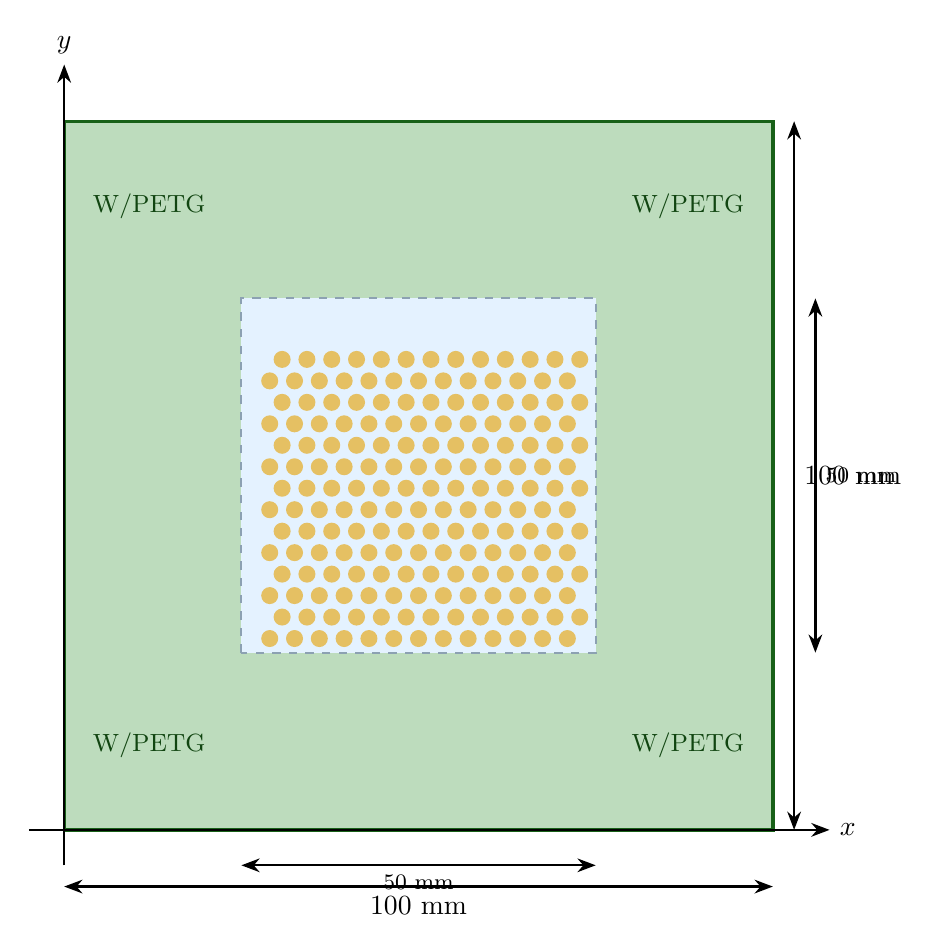
\begin{tikzpicture}[scale=0.9, >=Stealth]

% Plaque W/PETG (vue de dessus)
\fill[wpetg!30] (-5, -5) rectangle (5, 5);

% Cavite d'air
\fill[aircolor!50] (-2.5, -2.5) rectangle (2.5, 2.5);
\draw[thick, dashed, aircolor!70!black] (-2.5, -2.5) rectangle (2.5, 2.5);

% Grille de billes (arrangement hexagonal)
\def\d{0.35}
\def\dyh{0.303}

% Rangees de billes
\foreach \row in {0, 1, 2, 3, 4, 5, 6, 7, 8, 9, 10, 11, 12, 13} {
    \pgfmathsetmacro{\ypos}{-2.3 + \row * \dyh}
    \pgfmathsetmacro{\xoff}{mod(\row, 2) * 0.175}
    \foreach \col in {0, 1, 2, 3, 4, 5, 6, 7, 8, 9, 10, 11, 12} {
        \pgfmathsetmacro{\xpos}{-2.1 + \col * \d + \xoff}
        \fill[billeA!70] (\xpos, \ypos) circle (0.12);
    }
}

% Contour de la plaque
\draw[very thick, wpetg!70!black] (-5, -5) rectangle (5, 5);

% Axes
\draw[->, thick] (-5.5, -5) -- (5.8, -5) node[right] {$x$};
\draw[->, thick] (-5, -5.5) -- (-5, 5.8) node[above] {$y$};

% Cotations
\draw[<->, thick] (-5, -5.8) -- (5, -5.8) node[midway, below] {100 mm};
\draw[<->, thick] (-2.5, -5.5) -- (2.5, -5.5) node[midway, below] {\footnotesize 50 mm};
\draw[<->, thick] (5.3, -5) -- (5.3, 5) node[midway, right] {100 mm};
\draw[<->, thick] (5.6, -2.5) -- (5.6, 2.5) node[midway, right] {\footnotesize 50 mm};

% Labels
\node[wpetg!50!black, font=\small] at (-3.8, 3.8) {W/PETG};
\node[wpetg!50!black, font=\small] at (3.8, 3.8) {W/PETG};
\node[wpetg!50!black, font=\small] at (-3.8, -3.8) {W/PETG};
\node[wpetg!50!black, font=\small] at (3.8, -3.8) {W/PETG};

\end{tikzpicture}
\caption{Vue de dessus (XY) montrant la plaque W/PETG et la cavite centrale avec l'arrangement hexagonal des billes.}
\label{fig:vue_dessus}
\end{figure}

\newpage

%==============================================================================
\section{Empilement Hexagonal Compact des Billes}
%==============================================================================

\subsection{Principe de l'Empilement ABABA}

L'empilement hexagonal compact (HCP) utilise une sequence alternee de deux types de plans :
\begin{itemize}
    \item \textbf{Plans de type A} (plans 1, 3, 5) : position de reference
    \item \textbf{Plans de type B} (plans 2, 4) : decales de $(\delta x, \delta y)$ pour s'inserer dans les interstices
\end{itemize}

\begin{figure}[H]
\centering
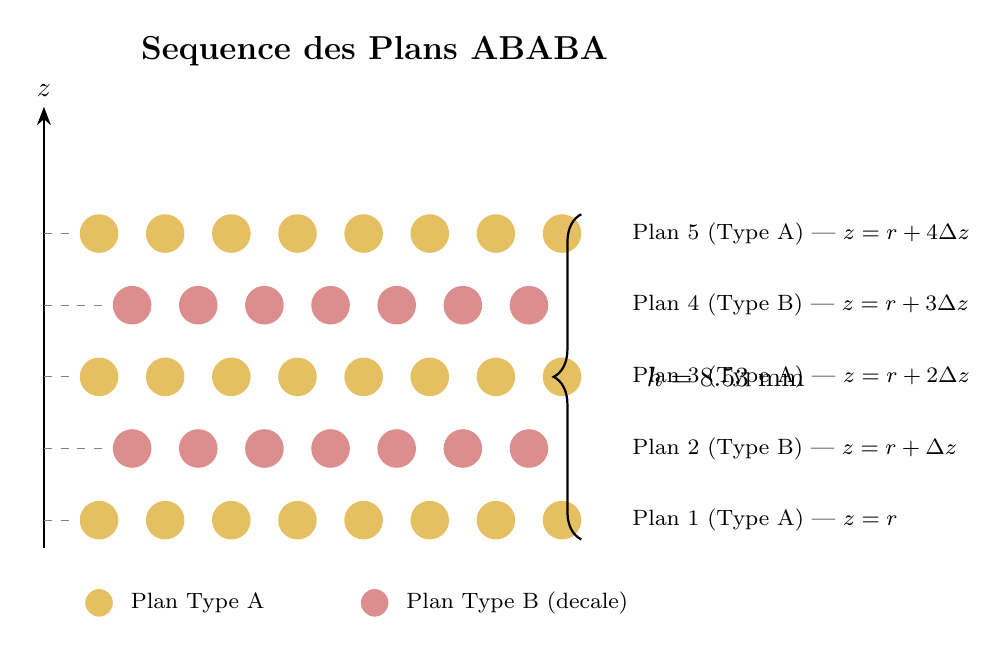
\begin{tikzpicture}[scale=0.7, >=Stealth]

% Titre
\node[font=\large\bfseries] at (6,9) {Sequence des Plans ABABA};

% Axe Z
\draw[->, thick] (0,0) -- (0,8) node[above] {$z$};

% Plan 1 (A)
\def\z{0.5}
\foreach \x in {1, 2.2, 3.4, 4.6, 5.8, 7, 8.2, 9.4} {
    \fill[billeA!70] (\x, \z) circle (0.35);
}
\node[right] at (10.5, \z) {\footnotesize Plan 1 (Type A) --- $z = r$};
\draw[dashed, gray] (0,\z) -- (0.6,\z);

% Plan 2 (B)
\def\z{1.8}
\foreach \x in {1.6, 2.8, 4.0, 5.2, 6.4, 7.6, 8.8} {
    \fill[billeB!70] (\x, \z) circle (0.35);
}
\node[right] at (10.5, \z) {\footnotesize Plan 2 (Type B) --- $z = r + \Delta z$};
\draw[dashed, gray] (0,\z) -- (1.2,\z);

% Plan 3 (A)
\def\z{3.1}
\foreach \x in {1, 2.2, 3.4, 4.6, 5.8, 7, 8.2, 9.4} {
    \fill[billeA!70] (\x, \z) circle (0.35);
}
\node[right] at (10.5, \z) {\footnotesize Plan 3 (Type A) --- $z = r + 2\Delta z$};
\draw[dashed, gray] (0,\z) -- (0.6,\z);

% Plan 4 (B)
\def\z{4.4}
\foreach \x in {1.6, 2.8, 4.0, 5.2, 6.4, 7.6, 8.8} {
    \fill[billeB!70] (\x, \z) circle (0.35);
}
\node[right] at (10.5, \z) {\footnotesize Plan 4 (Type B) --- $z = r + 3\Delta z$};
\draw[dashed, gray] (0,\z) -- (1.2,\z);

% Plan 5 (A)
\def\z{5.7}
\foreach \x in {1, 2.2, 3.4, 4.6, 5.8, 7, 8.2, 9.4} {
    \fill[billeA!70] (\x, \z) circle (0.35);
}
\node[right] at (10.5, \z) {\footnotesize Plan 5 (Type A) --- $z = r + 4\Delta z$};
\draw[dashed, gray] (0,\z) -- (0.6,\z);

% Accolade epaisseur totale
\draw[decorate, decoration={brace, amplitude=10pt, raise=5pt}, thick]
    (10,0.15) -- (10,6.05) node[midway, right=15pt] {$h = 8.53$ mm};

% Legende
\fill[billeA!70] (1,-1) circle (0.25);
\node[right] at (1.4,-1) {\footnotesize Plan Type A};
\fill[billeB!70] (6,-1) circle (0.25);
\node[right] at (6.4,-1) {\footnotesize Plan Type B (decale)};

\end{tikzpicture}
\caption{Vue en coupe XZ de l'empilement ABABA montrant l'alternance des plans.}
\label{fig:empilement_ababa}
\end{figure}

\subsection{Constantes Geometriques de l'Empilement}

\begin{table}[H]
\centering
\caption{Constantes de l'empilement hexagonal compact}
\begin{tabular}{llcc}
\toprule
\textbf{Constante} & \textbf{Formule} & \textbf{Expression} & \textbf{Valeur} \\
\midrule
Diametre bille & $d$ & -- & 2.0 mm \\
Rayon bille & $r = d/2$ & -- & 1.0 mm \\
Espacement Y (rangees) & $\Delta y_{\text{hex}}$ & $d \cdot \dfrac{\sqrt{3}}{2}$ & 1.732 mm \\[0.3cm]
Espacement Z (plans) & $\Delta z$ & $d \cdot \sqrt{\dfrac{2}{3}}$ & 1.633 mm \\[0.3cm]
Decalage X (plans B) & $\delta x_B$ & $\dfrac{d}{2}$ & 1.000 mm \\[0.3cm]
Decalage Y (plans B) & $\delta y_B$ & $\dfrac{d}{2\sqrt{3}}$ & 0.577 mm \\
\bottomrule
\end{tabular}
\end{table}

\subsection{Positions Z des Plans}

\begin{table}[H]
\centering
\caption{Positions verticales des 5 plans (base a $z = 0$)}
\begin{tabular}{cclc}
\toprule
\textbf{Plan} & \textbf{Type} & \textbf{Formule} & \textbf{Position $z$ (mm)} \\
\midrule
1 & A & $r$ & 1.000 \\
2 & B & $r + \Delta z$ & 2.633 \\
3 & A & $r + 2\Delta z$ & 4.266 \\
4 & B & $r + 3\Delta z$ & 5.899 \\
5 & A & $r + 4\Delta z$ & 7.532 \\
\bottomrule
\end{tabular}
\end{table}

L'epaisseur totale de l'empilement est :
\begin{equation}
h_{\text{total}} = r + 4 \cdot \Delta z + r = d + 4 \cdot d\sqrt{\frac{2}{3}} = 2 + 4 \times 1.633 = 8.53 \text{ mm}
\end{equation}

\newpage

%==============================================================================
\section{Vue 3D de l'Ensemble}
%==============================================================================

\begin{figure}[H]
\centering
\tdplotsetmaincoords{70}{120}
\begin{tikzpicture}[tdplot_main_coords, scale=0.8]

% Enveloppe (transparente)
\draw[very thin, gray, dashed] (-6,-6,0) -- (6,-6,0) -- (6,6,0) -- (-6,6,0) -- cycle;
\draw[very thin, gray, dashed] (-6,-6,8) -- (6,-6,8) -- (6,6,8) -- (-6,6,8) -- cycle;
\draw[very thin, gray, dashed] (-6,-6,0) -- (-6,-6,8);
\draw[very thin, gray, dashed] (6,-6,0) -- (6,-6,8);
\draw[very thin, gray, dashed] (6,6,0) -- (6,6,8);
\draw[very thin, gray, dashed] (-6,6,0) -- (-6,6,8);

% Plaque W/PETG (base)
\fill[wpetg!40, opacity=0.7] (-5,-5,2.5) -- (5,-5,2.5) -- (5,5,2.5) -- (-5,5,2.5) -- cycle;
\fill[wpetg!30, opacity=0.7] (5,-5,2.5) -- (5,5,2.5) -- (5,5,4.3) -- (5,-5,4.3) -- cycle;
\fill[wpetg!50, opacity=0.7] (-5,5,2.5) -- (5,5,2.5) -- (5,5,4.3) -- (-5,5,4.3) -- cycle;
\fill[wpetg!40, opacity=0.7] (-5,-5,4.3) -- (5,-5,4.3) -- (5,5,4.3) -- (-5,5,4.3) -- cycle;

% Cavite d'air (au centre)
\fill[aircolor!50, opacity=0.8] (-2.5,-2.5,2.93) -- (2.5,-2.5,2.93) -- (2.5,2.5,2.93) -- (-2.5,2.5,2.93) -- cycle;
\fill[aircolor!40, opacity=0.8] (2.5,-2.5,2.93) -- (2.5,2.5,2.93) -- (2.5,2.5,3.87) -- (2.5,-2.5,3.87) -- cycle;
\fill[aircolor!60, opacity=0.8] (-2.5,2.5,2.93) -- (2.5,2.5,2.93) -- (2.5,2.5,3.87) -- (-2.5,2.5,3.87) -- cycle;
\fill[aircolor!50, opacity=0.8] (-2.5,-2.5,3.87) -- (2.5,-2.5,3.87) -- (2.5,2.5,3.87) -- (-2.5,2.5,3.87) -- cycle;

% Billes (quelques-unes symboliques)
\foreach \x in {-2, -1, 0, 1, 2} {
    \foreach \y in {-2, -1, 0, 1, 2} {
        \shade[ball color=billeA!80] (\x, \y, 3.1) circle (0.15);
        \shade[ball color=billeB!80] (\x+0.5, \y+0.3, 3.4) circle (0.15);
        \shade[ball color=billeA!80] (\x, \y, 3.7) circle (0.15);
    }
}

% Detecteur dose (sphere)
\shade[ball color=watercolor!70] (0, 0, 10) circle (0.8);

% Axes
\draw[->, very thick] (0,0,0) -- (8,0,0) node[right] {$x$};
\draw[->, very thick] (0,0,0) -- (0,8,0) node[above] {$y$};
\draw[->, very thick] (0,0,0) -- (0,0,12) node[above] {$z$};

% Labels
\node[wpetg!50!black] at (0, -6.5, 3.4) {Plaque W/PETG};
\node[aircolor!50!black] at (4, 0, 3.4) {\footnotesize Cavite};
\node[blue] at (0, -2, 10) {\footnotesize Detecteur};

% Source
\shade[ball color=red!80] (0, 0, 0.5) circle (0.2);
\node[red!70!black] at (0, -1.5, 0.5) {\footnotesize Source};

\end{tikzpicture}
\caption{Vue 3D isometrique de la geometrie complete.}
\label{fig:vue_3d}
\end{figure}

\newpage

%==============================================================================
\section{Hierarchie des Volumes Geant4}
%==============================================================================

\begin{figure}[H]
\centering
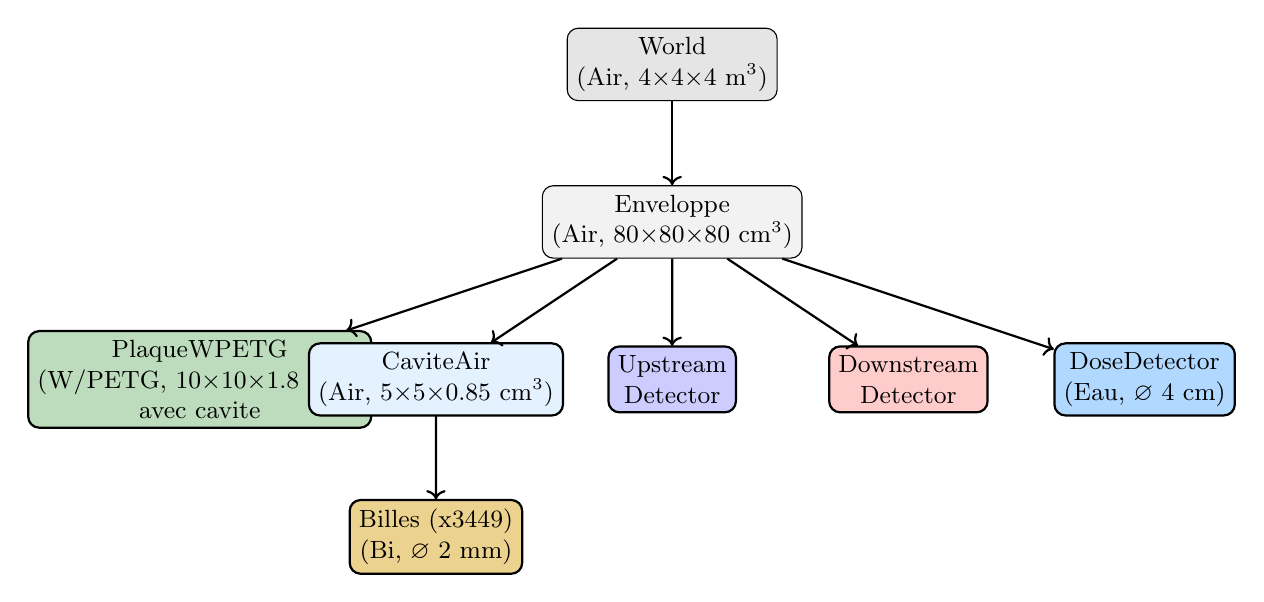
\begin{tikzpicture}[
    level 1/.style={sibling distance=6cm, level distance=2cm},
    level 2/.style={sibling distance=3cm, level distance=2cm},
    level 3/.style={sibling distance=2.5cm, level distance=2cm},
    every node/.style={rectangle, draw, rounded corners, align=center, font=\small},
    edge from parent/.style={draw, ->, thick}
]

\node[fill=gray!20] {World\\(Air, 4$\times$4$\times$4 m$^3$)}
    child {node[fill=enveloppe!50] {Enveloppe\\(Air, 80$\times$80$\times$80 cm$^3$)}
        child {node[fill=wpetg!30] {PlaqueWPETG\\(W/PETG, 10$\times$10$\times$1.8 cm$^3$)\\avec cavite}}
        child {node[fill=aircolor!50] {CaviteAir\\(Air, 5$\times$5$\times$0.85 cm$^3$)}
            child {node[fill=billeA!50] {Billes (x3449)\\(Bi, $\varnothing$ 2 mm)}}}
        child {node[fill=blue!20] {Upstream\\Detector}}
        child {node[fill=red!20] {Downstream\\Detector}}
        child {node[fill=watercolor!50] {DoseDetector\\(Eau, $\varnothing$ 4 cm)}}
    };

\end{tikzpicture}
\caption{Hierarchie des volumes logiques dans la simulation Geant4.}
\label{fig:hierarchie}
\end{figure}

\subsection{Description des Volumes}

\begin{enumerate}
    \item \textbf{World} : Volume mere principal, cube d'air de 4 m de cote.
    
    \item \textbf{Enveloppe} : Volume intermediaire contenant tous les elements de la simulation.
    
    \item \textbf{PlaqueWPETG} : Plaque de melange W/PETG (75\%/25\% en masse) avec une cavite centrale creee par soustraction booleenne (\texttt{G4SubtractionSolid}).
    
    \item \textbf{CaviteAir} : Volume d'air au centre de la plaque, contenant l'empilement de billes.
    
    \item \textbf{Billes} : Environ 3449 spheres de bismuth solide ($\varnothing$ 2 mm) arrangees en empilement hexagonal compact sur 5 plans.
    
    \item \textbf{UpstreamDetector / DownstreamDetector} : Plans de comptage pour mesurer le flux de particules avant et apres la plaque.
    
    \item \textbf{DoseDetector} : Sphere d'eau de 2 cm de rayon pour la mesure de dose absorbee.
\end{enumerate}

\newpage

%==============================================================================
\section{Resume des Masses et Densites}
%==============================================================================

\begin{table}[H]
\centering
\caption{Proprietes des materiaux et masses calculees}
\begin{tabular}{lcccc}
\toprule
\textbf{Element} & \textbf{Materiau} & \textbf{Densite} & \textbf{Volume} & \textbf{Masse} \\
 & & (g/cm$^3$) & (cm$^3$) & (g) \\
\midrule
Plaque W/PETG & W/PETG 75/25 & $\sim$4.5 & $\sim$176 & $\sim$790 \\
Cavite & Air & 0.0012 & 21.3 & $\sim$0.03 \\
Billes ($\times$3449) & Bismuth & 9.75 & $\sim$14.4 & $\sim$140 \\
Detecteur dose & Eau & 1.0 & 33.5 & 33.5 \\
\midrule
\textbf{Total plaque} & -- & -- & -- & $\sim$930 \\
\bottomrule
\end{tabular}
\end{table}

\begin{tcolorbox}[colback=green!5, colframe=green!70!black, title=\textbf{Avantages de cette Configuration}]
\begin{itemize}
    \item \textbf{Blindage efficace} : Le melange W/PETG fournit une attenuation importante des rayonnements gamma grace au tungstene (Z=74).
    \item \textbf{Absorption photoelectrique} : Les billes de bismuth (Z=83) au centre favorisent l'effet photoelectrique pour les photons de moyenne energie.
    \item \textbf{Geometrie bien definie} : Contrairement a la poudre, les billes ont une geometrie precise et reproductible.
    \item \textbf{Compacite elevee} : L'empilement hexagonal compact offre une fraction de remplissage theorique de 74\%.
\end{itemize}
\end{tcolorbox}

\end{document}
